% ---------------------------------------------------------------------------
% Factor-combination discovery as stochastic threshold group testing
%
% Manuscript source, written to the structure a general-interest methods
% journal expects (abstract, introduction, results, discussion, methods), which
% converts with little work to the alternatives:
%
%   Nature Communications / Cell Systems : as written.
%   PLOS Computational Biology           : add the Author summary (kept below),
%                                          move Methods before Results.
%   Bioinformatics                       : cut to 7 pages by dropping Section
%                                          2.5 and Figure 5.
%
% Build:  pdflatex main && bibtex main && pdflatex main && pdflatex main
% ---------------------------------------------------------------------------
\documentclass[11pt]{article}

\usepackage[utf8]{inputenc}
\usepackage[T1]{fontenc}
\usepackage[margin=1in]{geometry}
\usepackage{graphicx}
\usepackage{booktabs}
\usepackage{amsmath,amssymb}
\usepackage[expansion=false]{microtype}
\usepackage[labelfont=bf,font=small]{caption}
\usepackage[numbers,sort&compress]{natbib}
\usepackage[hidelinks]{hyperref}

\graphicspath{{../figures/}}

\title{\textbf{Factor-combination discovery is stochastic threshold group
testing: a counterfactual replay of the 2006 reprogramming screen}}

\author{Mashal Saleh Alkhalifah\thanks{Institute of Smart Cities, King
Abdulaziz City for Science and Technology (KACST), Riyadh, Saudi Arabia.
Correspondence: \texttt{mkhalifah@kacst.gov.sa}}}

\date{\today}

\begin{document}
\maketitle

\begin{abstract}
\noindent
Finding the small set of transcription factors that drives a cell-fate
conversion is expensive because each query is a wet-lab assay. The 2006 screen
that identified the four reprogramming factors consumed a documented 61
selection experiments under a fixed leave-one-out protocol. We show that this
class of screen is an instance of \emph{stochastic threshold group testing}: a
pool is negative below a lower threshold of essential factors, positive at or
above an upper threshold, and stochastic in the gap between, with the gap
response corresponding to the partial colony formation reported for
three-of-four pools. Placing the problem in that framework, and replaying the
screen on an oracle calibrated to the published assay figures, yields four
results. First, information-gain design recovers the hidden recipe in a median
of 10 experiments against 61, is cheaper in 300 of 300 paired replicates, and
matches the known $O(g^2 d \log n)$ order for the framework; an ablation with
identical inference but random pools needs 44, locating the gain in experiment
selection rather than in inference. Second, the advantage is regime-specific: a
classical model-free conjunctive search is twice as expensive at 24 candidates
but overtakes the Bayesian designer at 48, because random pool proposals stop
finding the recipe as the candidate list grows. Third, the method's only
structural failure is an assumed recipe cardinality, which fails
\emph{symmetrically and silently} --- zero success at 0.999 reported confidence
for both smaller and larger true recipes --- and is removed by treating
cardinality as a latent variable at a cost of one additional experiment.
Fourth, auditing the gap assumption against two measured combinatorial
perturbation datasets (171 combinations, two cell systems) finds a median
one-short response of 0.77 against the 0.10 the oracle assumes, placing the
calibration in the error direction our own sensitivity analysis identifies as
the dangerous one. We stress that the replay itself validates the search
procedure, not the oracle: the oracle is calibrated to the very screen being
replayed, so only the fourth result tests the model against data it was not
built from. We conclude that the gap response must be estimated per
assay rather than assumed, and that efficient experiment selection improves
cost while degrading the detectability of model error.
\end{abstract}

\section*{Author summary}
\small
When biologists search for the handful of genes that convert one cell type into
another, each guess costs weeks of laboratory work. We asked a counterfactual
question about a famous example: had the 2006 screen for the reprogramming
factors been planned adaptively, how many experiments would it have taken? On a
simulator calibrated to the original paper's numbers, about ten instead of
sixty-one. More useful than that number is where the approach breaks. The
problem turns out to be a known mathematical one --- threshold group testing ---
which supplies both a theoretical yardstick and a classical algorithm as a
competitor; that competitor wins once the candidate gene list passes about
forty, so the Bayesian approach earns its complexity only in the regime the
historical screen occupied. We also find a failure that matters for anyone
deploying these methods: if the number of genes in the recipe is fixed in
advance and that number is wrong, the search fails while reporting
near-certainty, whether the true recipe is larger or smaller. Finally, we check
the model's central assumption against real measurements and find it wrong in
the direction that causes exactly this kind of confident failure.
\normalsize

\section{Introduction}

A cell-fate conversion driven by defined factors is, computationally, a
subset-identification problem: of $n$ candidates, an unknown subset $R$ of size
$k$ is sufficient, and the task is to find $R$. What makes it hard is not the
size of the space but the price of a query. Each query is a transduction
experiment with a biological readout, so budgets are counted in tens.

The canonical instance is the screen of \citet{takahashi2006}, extended to human
cells the following year \citep{takahashi2007}. Twenty-four candidates were
selected from the literature; the readout was the number of
drug-resistant colonies surviving Fbx15/G418 selection; and the search followed
a fixed protocol --- each factor alone, the full pool, leave-one-out from the
pool, then leave-one-out from the surviving subset --- consuming $2n + 13 = 61$
experiments at $n = 24$ regardless of what the data said.

Adaptive experimental design \citep{lindley1956, chaloner1995, rainforth2024}
should improve on a protocol fixed in advance, and in perturbation biology
several groups have shown that it does \citep{zhang2023, tosh2025}. What has not been established is
the counterfactual for a specific documented discovery: not predictive accuracy
over an adaptively collected dataset, but the number of wet-lab experiments
needed to reach a known answer under the assay actually used. The 2006 screen
is a good vehicle precisely because its experiment count is in the public
record.

Our second contribution is a reclassification. The colony assay is not generic
combinatorial search: a pool produces colonies efficiently only when it contains
all of $R$, weakly when it contains all but one, and not at all otherwise. In
group-testing language \citep{dorfman1943, aldridge2019}, a test is negative at or below a
lower threshold $l$, positive at or above an upper threshold $u$, and stochastic
in the gap $g = u - l - 1$. This is threshold group testing
\citep{damaschke2006} in its stochastic form \citep{chan2013}, with $u = k$,
$l = k - 2$ and $g = 1$. The reclassification is load-bearing rather than
decorative: it supplies a theoretical yardstick for the achievable test count
and classical algorithms as baselines, and both change the conclusions one would
otherwise draw.

\paragraph{Related work.} Four literatures meet here, and the closest work in
each sits a measurable step away from this one.

\emph{Group testing} supplies the problem class and its bounds, from the
original pooled-screen argument \citep{dorfman1943} through the modern
information-theoretic treatment \citep{aldridge2019}. The variant that matches
this assay is threshold group testing \citep{damaschke2006} in its stochastic
form \citep{chan2013}, and designs for it continue to improve
\citep{bui2024}. Those designs are parameterised by the threshold $u$: it is
given, and the algorithm is built around it. Here $u = |R|$ is exactly what the
experimenter does not know, which is the gap Section~\ref{sec:cardinality}
addresses. Group testing is also being applied to biology right now
\citep{talamanca2026}, but in its disjunctive form --- a pool is positive if it
contains any positive item --- and largely non-adaptively, whereas a
reprogramming pool is positive only if it contains \emph{all} of the recipe.

\emph{Bayesian experimental design} supplies the criterion
\citep{lindley1956, chaloner1995, rainforth2024}. Applied to perturbation
biology, it has been used to choose genetic interventions \citep{zhang2023} and
combination drug screens \citep{tosh2025}, and recent work learns an acquisition
policy amortised over more than a thousand historical CRISPR screens
\citep{edwards2026} or selects gene pairs with a predictive model in the loop
\citep{qin2025}. These are evaluated on hit-recovery or predictive accuracy at a
fixed budget fraction. None asks the counterfactual question of this paper: how
many experiments a documented discovery would have taken, measured against the
count that discovery actually consumed.

\emph{Prediction rather than design} is the third line: ranking reprogramming
factors from expression and network data \citep{rackham2016}, scoring
transcription-factor combinations from single-cell multiomics
\citep{tfcomb2025}, and predicting outcomes of unseen multi-gene perturbations
\citep{roohani2022}. The closest of these even frames its accuracy in
experiment-count terms --- a cocktail ranked fiftieth implies fifty experiments
--- but the ranking is static: it does not condition on results as they arrive,
and the count is a corollary of the ranking rather than a measured search cost.
Such models are nonetheless the natural replacement for the oracle used here,
which is the direction the virtual-cell programme points \citep{bunne2024}.

\emph{Validation of adaptive policies} is the fourth. Held-out evaluations of
selective measurement rules in biological screens have found that the evidence
often fails to justify adopting them over a fixed plan \citep{bi2026}, a
finding that sits naturally beside Section~\ref{sec:stopping}: efficiency and
error detectability pull in opposite directions.

Against that background the contributions of this paper are the counterfactual
against a historical experiment count, the regime boundary against a classical
algorithm, the treatment of an unknown threshold in a threshold-group-testing
assay, and a check of the assay model's central assumption against measured
data.

We state plainly what this study is not. The oracle is a simulator calibrated to
summary figures, not an assay and not a fit to raw data; Section~\ref{sec:real}
is where measured data enters, and it refutes part of the calibration. No claim
about cellular biology follows from any result here.

One inference in particular is unavailable to us, and we flag it because it is
the natural reading of a replay. \textbf{Recovering the Yamanaka factors is not
evidence that the oracle is right.} The oracle was built from the numbers that
screen reported, and the recipe is a truth we planted in it; finding that recipe
therefore tests the search procedure and nothing else. Treating the recovery as
validation of the model would be circular. What the replay measures is the cost
of a search strategy under a documented fitness function, against a published
experiment count --- the same sense in which running a heuristic on a
solved instance measures the heuristic, not the instance. Validation of the
model happens only once in this paper, in Section~\ref{sec:real}, where its
central parameter is compared against measurements it was not fitted to, and
fails.

\section{Results}

\subsection{Cost against the historical record}
\label{sec:main}

\begin{figure}[t]
  \centering
  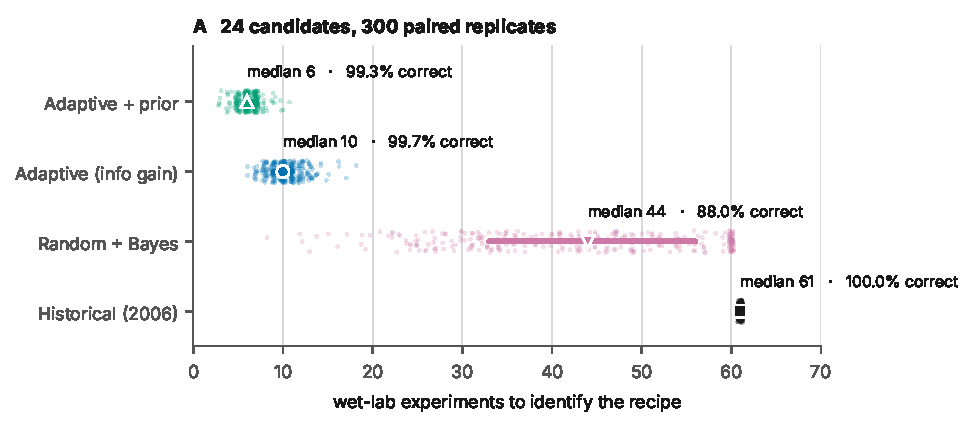
\includegraphics[width=0.86\textwidth]{fig1_main_comparison.pdf}
  \caption{\textbf{Wet-lab cost of four strategies at 24 candidates, 300 paired
  replicates.} Each point is one replicate; bars span the interquartile range,
  markers give medians. The ablation --- the same exact posterior and stopping
  rule with pools drawn at random --- separates the contribution of experiment
  selection from that of inference; its pile-up at 60 is the budget ceiling.}
  \label{fig:main}
\end{figure}

Over 300 replicates (Fig.~\ref{fig:main}), the historical protocol consumes its
fixed 61 experiments; information-gain design needs a median of 10 (95\% CI
[10, 10]; mean 10.3; worst replicate 18) and recovers the exact recipe in
99.7\% of runs; a literature prior reduces this to 6. Paired against the
historical protocol, the adaptive designer is cheaper in 300 of 300 replicates.

Two controls matter more than the headline. The ablation needs a median of 44
experiments and recovers the recipe in 88.0\% of runs; paired, the difference is
32.7 experiments (permutation $p < 10^{-4}$), with the adaptive designer cheaper
in 298 of 300 replicates. The saving comes from informative experiment
selection, not from Bayesian updating. The literature prior buys speed and
nothing else: $-4.1$ experiments ($p < 10^{-4}$) with no detectable accuracy
difference (McNemar $p = 1.0$).

The measured cost should be read against theory rather than against the 2006
protocol alone. For stochastic threshold group testing, test counts of order
$g^2 d \log n$ are achievable \citep{chan2013}; at $g = 1$, $d = 4$, $n = 24$
that is $\approx 13$, consistent with the observed median of 10. The 84\% saving
is therefore not a surprising empirical finding but the expected consequence of
replacing a $\Theta(n)$ protocol with one operating at the model's known order.
That is itself the point: the gap between what the 2006 screen spent and what
was achievable was derivable from theory contemporaneous with it.

\subsection{The advantage is regime-specific}
\label{sec:scaling}

\begin{figure}[t]
  \centering
  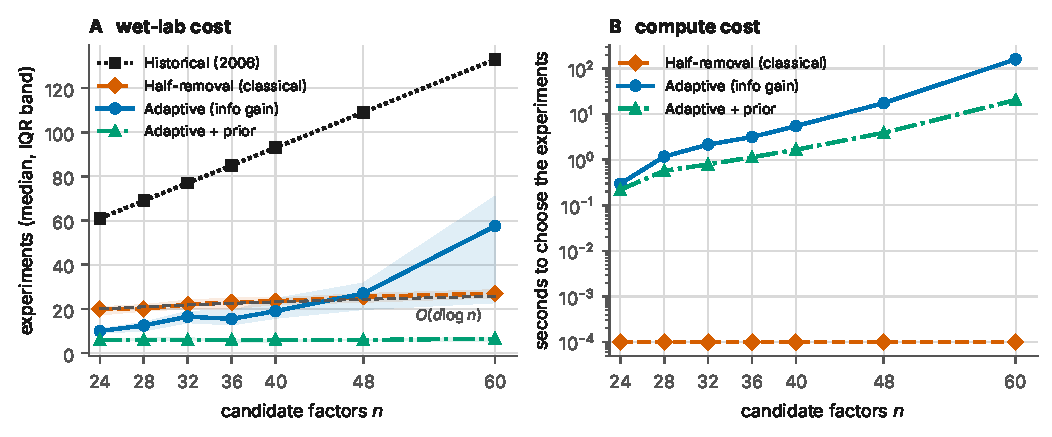
\includegraphics[width=\textwidth]{fig2_scaling.pdf}
  \caption{\textbf{Growth with candidate-list size.} (A) Wet-lab cost, medians
  with interquartile bands, against the $O(d\log n)$ reference curve scaled at
  the smallest list. (B) Compute spent choosing experiments, log scale. The
  classical half-removal search recovers logarithmic growth at negligible
  compute; the Bayesian designer does not, and the two cross at 48 candidates.}
  \label{fig:scaling}
\end{figure}

Yamanaka's 24 candidates were themselves the product of a literature filter, so
a method that works only after such filtering is of limited use.
Figure~\ref{fig:scaling} varies the list from 24 to 60 factors, i.e.\ hypothesis
spaces from $10{,}626$ to $487{,}635$.

The Bayesian designer's wet-lab cost grows as $n^{1.8}$, not logarithmically,
and its advantage over the historical protocol decays from 84\% to 57\%. The
classical half-removal search shows the opposite pattern: twice as expensive at
$n = 24$ (20 versus 10 experiments), it grows as $n^{0.4}$ and the two curves
cross at $n = 48$ (26 versus 27). Because the classical search carries no model
of the assay, this localises the deficiency: not in the inference and not in the
problem, but in proposal generation. Random pools of size 2--12 contain all four
essential factors with probability falling as $n^{-4}$, so as the list grows the
designer evaluates information gain ever more accurately over proposals ever
less likely to be informative. The remedy is a better proposal distribution, and
the classical algorithm is in effect one.

Neither method dominates. The classical search pays for its simplicity in
reliability: its success rate falls from 100\% to 83\% as $n$ grows to 60, for a
physical reason rather than an algorithmic one. The pool-size penalty drags a
full 60-factor pool down to about 6 expected colonies, so the positive control
the algorithm starts from approaches the noise floor. The Bayesian designer
holds 100\% at every size because it reasons from the whole count distribution
rather than from one threshold. Compute separates them further: 159~s per run at
$n = 60$ against under a millisecond.

The $k+1$ overlap-class collapse (Section~\ref{sec:methods-inference}) makes the
cost of scoring a proposal independent of posterior concentration, but it
remains linear in the enumerated space, and the number of rounds grows too;
empirically design cost grows as $H^{1.5}$ in the hypothesis count $H$. Exact
enumeration is the binding constraint beyond about 60 candidates. One curve in
Figure~\ref{fig:scaling} must be read with care: the literature-prior variant
appears flat in $n$ only because prior quality is held constant, up-weighting
eight factors regardless of $n$. A longer candidate list implies a less
informative prior, so that curve is an upper bound conditional on prior quality,
not a prediction.

\subsection{Model error: absent signal versus wrong signal}
\label{sec:calibration}

\begin{figure}[t]
  \centering
  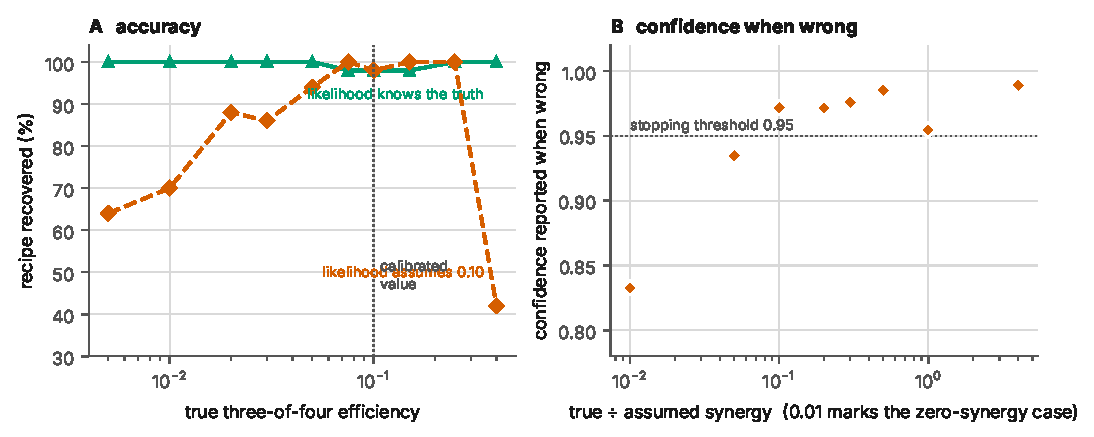
\includegraphics[width=\textwidth]{fig3_calibration.pdf}
  \caption{\textbf{Gap response and calibration error.} (A) Recovery rate as the
  true three-of-four efficiency $\rho$ varies, with the likelihood either
  informed of it or holding the calibrated 0.10. (B) Confidence reported in runs
  that returned a wrong recipe, against the ratio of true to assumed $\rho$ (the
  leftmost point is the zero-gap case).}
  \label{fig:calibration}
\end{figure}

The graded three-of-four signal is the gap response of the threshold model, and
it is natural to suppose the search depends on it. Separating the signal's
presence from the searcher's belief about it shows otherwise
(Fig.~\ref{fig:calibration}A). With the gap response removed entirely
($\rho = 0$) and the likelihood informed of this, the recipe is still recovered
in 100\% of runs at a median of 22 experiments: the search degenerates to pure
group testing, pays a factor of 2.2 for the lost gradient, and remains 64\%
cheaper than the historical protocol. The same oracle with a searcher that keeps
believing $\rho = 0.10$ succeeds in 52\% of runs. Absence of graded synergy is a
calibration error, not a structural barrier.

What binds is the magnitude of the error, asymmetrically. Under-estimating the
gap response fivefold still recovers the recipe in 70\% of runs, while
over-estimating it fourfold drops recovery to 42\% --- and reports confidence
0.989 while doing so. Conservative calibration is the safer error direction,
which matters because the gap response is exactly the quantity a pilot
experiment estimates poorly.

\subsection{Assumed cardinality: a symmetric, silent failure}
\label{sec:cardinality}

\begin{figure}[t]
  \centering
  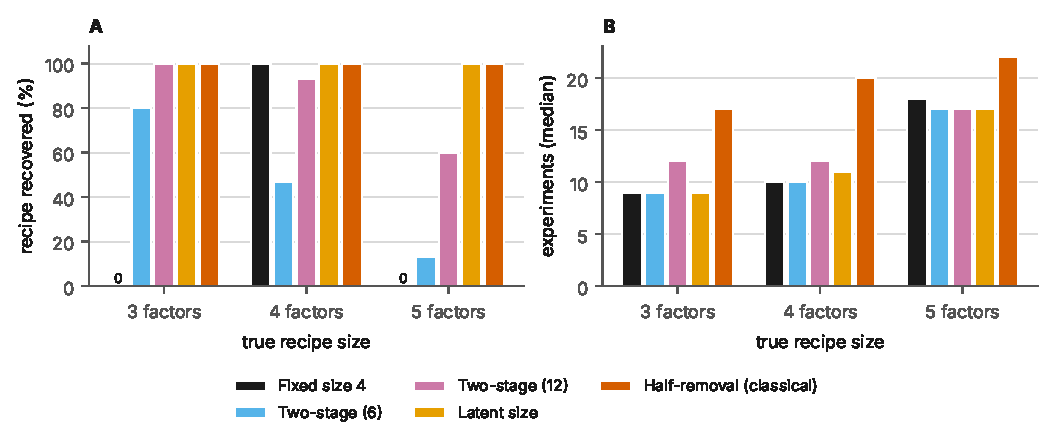
\includegraphics[width=\textwidth]{fig4_cardinality.pdf}
  \caption{\textbf{Unknown recipe size, several treatments, three truths.}
  (A) Exact-recipe recovery. (B) Cost. Fixing the size at four fails completely
  when the truth is three or five; estimating the size in a first stage and
  committing to it inherits the failure whenever the estimate is wrong; carrying
  size as a latent variable, or dispensing with a size representation
  altogether, does not.}
  \label{fig:cardinality}
\end{figure}

Every result above assumes the searcher knows $k = 4$. Relaxing that assumption
exposes the method's one genuinely structural failure
(Fig.~\ref{fig:cardinality}). A designer fixed at four factors recovers a
three-factor recipe in 0\% of runs and a five-factor recipe in 0\% of runs, and
in both cases reports a mean posterior confidence at or above 0.99 on the wrong
answer. The failure is symmetric: searching for more factors than exist is as
fatal as searching for fewer, because the fixed designer appends a spurious
factor to a correct core and then concludes. This is not a failure of the data
but of a hypothesis space that cannot represent the truth, and the posterior is
confident precisely because every hypothesis it can represent is wrong by the
same margin.

Treating cardinality as latent removes it. Recovery is 100\% at true sizes
three, four and five; the correct size carries posterior mass 0.995 or above in
all three cases; and the premium on the four-factor case the fixed designer was
built for is $+0.9$ experiments (paired $p = 0.0036$). The latent treatment also
returns a diagnostic the fixed designer cannot produce even in principle: a
posterior over recipe size, which is what would tell an experimenter that their
assumed cardinality was wrong.

Two comparators place this result. The classical answer to unknown $|R|$ is to
estimate the count in a first stage and then commit to it \citep{bshouty2018}.
That baseline inherits the failure whenever the first stage errs, and it errs
often: with a six-experiment first stage it commits to the wrong size in 53\% of
four-factor runs and 87\% of five-factor runs, recovering the recipe in 47\% and
13\% of them; doubling the first stage to twelve experiments reduces the wrong
commitments to 7\% and 40\%, for 93\% and 60\% recovery, at a cost of
$+1.7$ experiments on the four-factor case ($p = 0.005$). Carrying the size
posterior throughout instead of committing to it is thus not redundant
machinery: it is what converts a 60\% method into a 100\% one at no measurable
premium ($+0.5$ experiments, $p = 0.53$). The model-free half-removal search
sidesteps the question entirely, since it never represents a size, and recovers
all three sizes without modification --- for $+9.7$ experiments
($p < 10^{-4}$), roughly double. Cardinality is therefore a liability of the
parametric approach specifically, not of the problem.

\subsection{The stopping rule, and a trade-off between efficiency and
detectability}
\label{sec:stopping}

\begin{figure}[t]
  \centering
  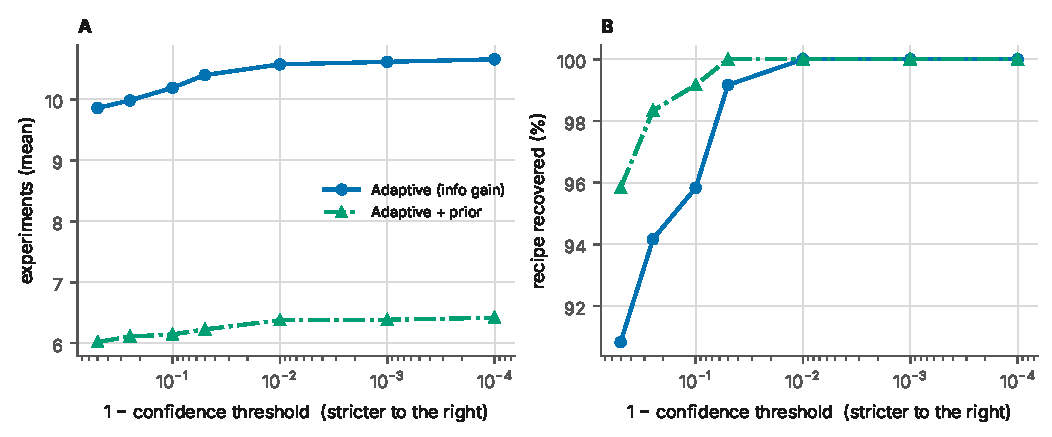
\includegraphics[width=\textwidth]{fig5_stopping_rule.pdf}
  \caption{\textbf{The price of certainty.} (A) Mean experiments and (B)
  recovery rate as the stopping threshold tightens from 0.50 to 0.9999. Cost is
  nearly flat while accuracy improves, because posterior confidence jumps at the
  decisive experiment rather than climbing gradually.}
  \label{fig:stopping}
\end{figure}

A Bayesian stopping rule is usable only if its confidence means what it says,
since in a real campaign there is nothing to check it against. Sweeping the
threshold from 0.50 to 0.9999 (Fig.~\ref{fig:stopping}), the stated confidence
never exceeds the observed recovery rate by more than its Wilson interval
permits (largest discrepancy $+0.025$), and tightening by four orders of
magnitude costs 0.8 experiments on average while never moving the median. The
practical recommendation is to run at 0.999 or tighter.

That flatness is the mechanism behind a pattern visible throughout. Confidence
does not accumulate gradually; it jumps at the decisive experiment, so there is
no intermediate regime in which the searcher can report that it is not sure yet.
When the model is wrong, high confidence therefore arrives just as promptly on
the wrong answer: the adaptive designer's mean confidence when wrong is 0.955
against 0.423 for the random-pool ablation; an over-estimated gap response fails
at 0.989; a cardinality mismatch fails at 0.999. The designer is well calibrated
\emph{inside its model}, and that does not protect it when the model is wrong.
Efficient experiment selection improves cost and degrades the detectability of
model error at the same time, because a procedure that gathers consistent
evidence quickly gathers it quickly for a wrong hypothesis too.

\subsection{The gap assumption against measured data}
\label{sec:real}

\begin{figure}[t]
  \centering
  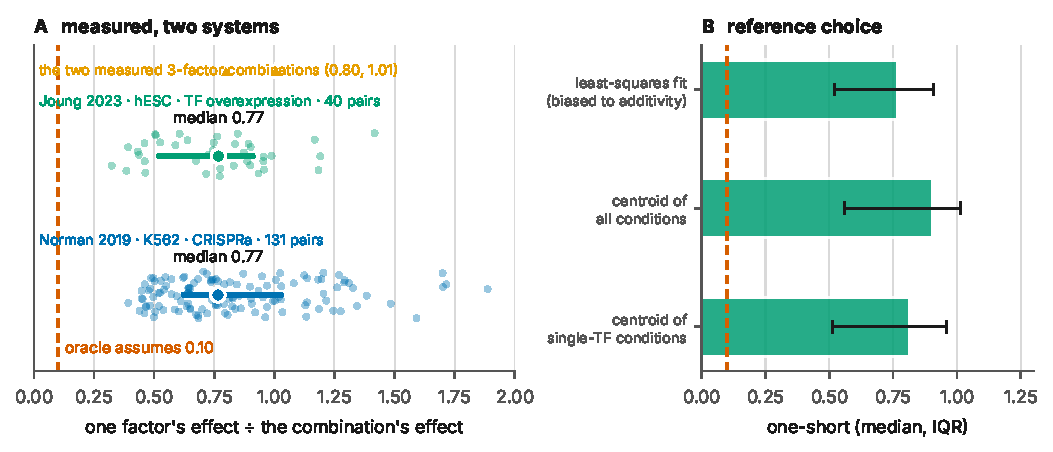
\includegraphics[width=\textwidth]{fig6_real_data.pdf}
  \caption{\textbf{What one factor of a measured combination reproduces.}
  (A) The ratio $\lVert\delta_{\text{one short}}\rVert /
  \lVert\delta_{\text{combination}}\rVert$ for 131 gene pairs in K562
  \citep{norman2019} and 40 transcription-factor pairs in human embryonic stem
  cells \citep{joung2023}, with the two measured three-factor combinations
  marked. The oracle assumes 0.10. (B) The hESC subset has no unperturbed
  control, so three references are reported; the conclusion does not depend on
  the choice.}
  \label{fig:real}
\end{figure}

Every result above is conditional on gap structure of the assumed shape
existing. Single-cell perturbation screens now cover enough combinations to
check it directly \citep{replogle2022, peidli2024}, and two of them carry the
pairs and singles the measurement needs. For a perturbation $p$ with
pseudobulk profile $x_p$ and reference $x_0$, write
$\delta_p = x_p - x_0$; for each combination whose one-short constituents were
also profiled, we measure
\begin{equation}
  \text{one-short} =
  \frac{\max_{c}\ \lVert \delta_c \rVert}{\lVert \delta_{\text{combination}} \rVert},
  \label{eq:oneshort}
\end{equation}
the empirical analogue of $\rho$, whose calibrated value is 0.10.

In \citet{norman2019} --- K562, CRISPRa, 131 pairs with both singles measured
--- the median is \textbf{0.77} (IQR 0.62--1.03), and \textbf{no pair of the 131}
falls below 0.20. In the combinatorial subset of \citet{joung2023} --- human
embryonic stem cells, transcription-factor overexpression, 40 TF--TF pairs ---
the median is \textbf{0.77} (IQR 0.52--0.91) under a reference fitted by least
squares, 0.91 and 0.82 under two alternative references, with no pair below 0.20
under any of them (Fig.~\ref{fig:real}B). The two measured three-factor
combinations give 0.80 and 1.01.

The result is not an artefact of measuring effect size by a Euclidean norm.
Repeating the Norman analysis with threshold-like functionals --- the number of
genes moving more than 0.25 or 0.5 in log space --- lowers the median to 0.48
and 0.50 and raises the fraction below 0.20 to 25\% and 22\%, but no functional
produces a median near 0.10.

Two further observations. First, departures from additivity are common but
modest in magnitude: in Norman the median ratio of the pair's effect to the sum
of its singles is 0.91, with 47\% of pairs sub-additive and 27\% super-additive,
and only 28\% of pairs have an additivity residual exceeding its own sampling
noise, estimated by regressing squared residuals on
$1/n_{AB} + 1/n_A + 1/n_B$. Second, the two systems differ in \emph{where} the
interaction lives: the median $R^2$ of a pair on its two singles is 0.86 in
K562 but 0.64 in hESCs, so combinations in the stem-cell system leave the plane
spanned by their constituents more, while their magnitudes remain near-additive.

The implication is specific. Our calibrated $\rho = 0.10$ is five- to eightfold
sharper than measurement supports, and Section~\ref{sec:calibration} shows that
over-estimating the gap response is precisely the direction in which the
designer fails silently. A designer calibrated as ours is would therefore be
expected to fail confidently on these systems, while the same designer informed
of the true $\rho$ succeeds in 98--100\% of runs at every value tested,
including $\rho = 0$. The gap response must be estimated, not assumed.

The constructive reading is that the oracle should be replaced rather than
recalibrated: a predictive model fitted to measured perturbation outcomes
\citep{roohani2022}, or the broader virtual-cell programme
\citep{bunne2024}, would supply a gap response estimated from data rather than
assumed, and the designer would inherit whatever accuracy that model has. The
experiments above then become the specification for how accurate it must be:
within a factor of two on the gap response, and honest about recipe size.

One boundary deserves emphasis. Both datasets read out the transcriptome, while
the 2006 assay reads out a rare discrete phenotype --- a colony forms or does
not --- which is a thresholded functional of cell state and may well be far
sharper than transcriptome displacement. The audit therefore refutes the
assumption for expression-level objectives and constrains, rather than settles,
the phenotype case. Settling it requires a combinatorial screen with a
phenotypic readout, which to our knowledge does not exist at the scale needed.

\section{Discussion}

Four conclusions survive the controls, and they are narrower than the headline
saving.

The saving is real but unsurprising once the problem is named. Recognising the
colony assay as stochastic threshold group testing with $g = 1$ supplies the
achievable order, $O(g^2 d\log n)$, and the observation that the 2006 protocol
operated at $\Theta(n)$. The contribution is not the adaptive designer but the
quantification: how much of that theoretical gap is realisable under the assay's
noise, with the historical count as the reference.

The Bayesian apparatus earns its place only in a regime. At the scale the
historical screen occupied it is twice as efficient as a classical conjunctive
search; beyond 48 candidates it is worse in experiments and five orders of
magnitude worse in compute, while remaining more reliable. Any application to
larger candidate lists should either repair the proposal distribution, plausibly
by borrowing the classical algorithm's structure, or use the classical algorithm
with the Bayesian machinery reserved for the final discrimination.

For deployment, the cardinality result is the most actionable: a parametric
designer that fixes recipe size fails silently and symmetrically, the standard
two-stage remedy inherits the failure, and latent-cardinality inference removes
it for about one extra experiment while supplying a size posterior that makes
the error visible. Given the general pattern that efficient design suppresses
the signature of model error, cheap diagnostics of this kind are not optional
extras.

Finally, the real-data audit turns the study's main caveat into a result. The
assumption that a one-short pool yields a tenth of the full response is not
supported in either measured system; the measured value is close to 0.8. Since
over-estimating that response is the error direction that produces confident
failure, the operational rule follows directly: measure the gap response in a
pilot, calibrate conservatively, and treat a designer that has not done so as
untrustworthy regardless of what its posterior reports.

\paragraph{What these experiments specify.} Read together, the results are less
a study of one historical screen than a specification for the evaluator that any
such search runs inside. A search procedure consumes an evaluator, and the
questions this paper answers are the ones an evaluator must satisfy before
searching inside it pays: its gap response must be accurate to within about a
factor of two, with under-estimation the safer error
(Section~\ref{sec:calibration}); it must expose uncertainty over structure, not
only a score, because a model that cannot represent the right recipe size fails
silently at 0.999 confidence (Section~\ref{sec:cardinality}); and its stopping
confidence is trustworthy only to the extent its own model is
(Section~\ref{sec:stopping}). Those are testable requirements, and they apply to
a learned model of cell state as much as to the calibrated oracle used here.

The measured data adds a fourth requirement and relaxes one assumption. An
evaluator fitted to expression data will present a graded, near-additive
landscape rather than the sharp threshold the 2006 assay suggests
(Section~\ref{sec:real}), which is easier to search, not harder --- but it also
means the gap response has to be estimated from a pilot rather than inherited
from a published figure.

\paragraph{Where the method ends and another begins.} The scaling result marks
a boundary that matters beyond this benchmark. Exact enumeration over
hypotheses is what makes the posterior cheap, and it is also what fails: by 60
candidates the design step costs 159~s per run and the wet-lab saving has
halved. A reprogramming search over the roughly 1{,}600 human transcription
factors is three orders of magnitude past that, so the approach used here
cannot be carried to it by tuning. What the classical comparator shows is that
the missing ingredient is proposal generation, which is precisely what
population-based search supplies: a set of candidates evolved from the
currently promising ones rather than enumerated or drawn at random. The natural
successor to this work is therefore not a larger posterior but a search whose
proposals are generated and whose evaluator is a learned model, with the
requirements above as its acceptance criteria.

\paragraph{Next steps.} Four follow from the results, in order of what each
would settle. First, replace the calibrated oracle with a retrospective one
built directly from measured combinatorial data, turning every count reported
here from a property of a model into a measurement. Second, rebuild the
proposal distribution along the lines the classical comparator suggests and
test whether logarithmic scaling is recovered, which is the difference between
diagnosing the defect and repairing it. Third, make the gap response a latent
parameter estimated during the search rather than a fixed constant, which the
real-data audit shows is the assumption most likely to be wrong in deployment.
Fourth, and most open: the threshold-group-testing literature parameterises its
designs by a \emph{known} threshold, while the quantity an experimenter lacks is
exactly that threshold. Bounds for threshold group testing with unknown $u$
would place the cardinality result of Section~\ref{sec:cardinality} on a
theoretical footing rather than an empirical one.

\paragraph{Limitations.} The oracle is a simulator calibrated to published
summary figures, so its numbers are properties of a stated model; the design of
the comparisons, not the realism of the oracle, carries the conclusions. The
audit datasets read out expression rather than a rare phenotype, which is the
readout the historical assay used; the evaluator-quality lesson of
\citet{okita2007}, where a better selection marker changed which colonies counted
as success, is the biological form of the same concern. The historical protocol is
reconstructed from
the paper's description rather than laboratory records. The latent-cardinality
designer widens its assumption to sizes 3--6 rather than eliminating it, so a
seven-factor truth would reproduce the original failure. Exact enumeration
limits the approach to candidate lists of order $10^2$, which excludes the
genome-scale setting where a reprogramming screen would benefit most.

\section{Methods}
\label{sec:methods}

\subsection{Oracle}

A hidden essential set $R \subseteq \{1,\dots,n\}$, $|R| = k$, is drawn
uniformly. For a transduced pool $S$, the colony count is a Poisson draw,
\begin{equation}
  y(S) \sim \mathrm{Poisson}\!\left(\lambda(S)\right), \qquad
  \lambda(S) = B\, \phi\!\left(|S \cap R|\right)
  \exp\!\left(-\delta \max(0, |S| - k)\right),
  \label{eq:oracle}
\end{equation}
with $\phi(k) = 1$, $\phi(k-1) = \rho$ and $\phi(j) = 0$ for $j < k - 1$.
Calibration targets from \citet{takahashi2006}: a clean four-factor pool yields
about 45 colonies ($B = 45$); a three-of-four pool yields a small number lacking
full ES-like morphology ($\rho = 0.10$, about 4 colonies); per-cell efficiency
falls as more factors are transduced, which is why the reported 10-factor subset
outperformed the full 24 ($\delta = 0.0357$, giving 36 and 22 colonies). In
threshold-group-testing terms, $u = k$, $l = k - 2$, $g = 1$, and $\rho$ is the
gap response.

\subsection{Inference}
\label{sec:methods-inference}

The hypothesis space is every $k$-subset of the candidates
($\binom{24}{4} = 10{,}626$ in the calibrated case), small enough for an exact
posterior with no sampling. The next pool maximises expected information gain
\citep{lindley1956},
$\mathrm{EIG}(S) = H[p(y \mid S)] - \mathbb{E}_{h}\,H[p(y \mid S, h)]$,
over 120--260 random pools of size 2--12 plus pools assembled from the most
probable factors. The count distribution depends on a hypothesis only through
$|S \cap h|$, which takes $k + 1$ values, so likelihood and information gain
collapse onto $k+1$ overlap classes and the cost of scoring a proposal is
independent of posterior concentration. The search stops when the leading
hypothesis exceeds $\tau$ (0.95 unless stated) or the budget is exhausted.

For unknown cardinality the space becomes every subset of size 3--6
($189{,}750$ at $n = 24$) and the rate depends on a hypothesis through the pair
$(|h|, |S \cap h|)$, giving 22 reachable classes, so the same collapse applies
one dimension up.

\subsection{Strategies and baselines}

\textbf{Historical protocol.} $n$ single-factor experiments, the full pool, $n$
leave-one-out experiments, the surviving 10-factor pool, 10 leave-one-out
experiments, and a confirmation: $2n + 13$, non-adaptive.
\textbf{Adaptive design}, with a uniform prior, and \textbf{with a literature
prior} up-weighting eight factors (the true ones plus decoys), whose quality is
varied over coverage, breadth and strength in a separate experiment.
\textbf{Random pools with Bayesian updating} is the ablation: identical
inference, pools drawn at random.
\textbf{Half-removal search} is the conjunctive analogue of binary splitting,
carrying no model beyond a positivity threshold and no representation of recipe
size: half the undecided factors are removed and the pool retested; if it
remains positive every removed factor was inessential and the candidate set
halves, and if it turns negative the removed half contains an essential factor,
found by binary search. Its one hyperparameter, the positivity threshold, is the
geometric mean of the assumed full and gap rates at the pool size tested, so it
carries the same calibration error as the Bayesian designer.
\textbf{Two-stage cardinality estimation} spends a fixed budget (6 or 12
experiments) estimating the count, then commits to it \citep{bshouty2018}.
\textbf{Latent-cardinality design} carries size and identity in one posterior.

\subsection{Campaign and statistics}

Results come from independent replicates recorded individually, so that all
aggregation is reproducible without re-simulation; strategies within an
experiment share hidden recipes and noise seeds, making every comparison paired.
Cost is summarised by medians with interquartile ranges, because experiment
counts are integer, bounded below and right-skewed. Median intervals are
percentile bootstrap ($20{,}000$ resamples); proportions use Wilson score
intervals, which retain width at 0\% and 100\%. Paired cost comparisons use a
two-sided paired permutation test on the mean difference ($20{,}000$ sign
flips); paired accuracy comparisons use an exact McNemar test. Success
thresholds are estimated by logistic regression in $\log_{10}$ of the varied
parameter and reported only when the crossing lies inside the tested range. The
statistics layer is implemented in NumPy and checked against closed-form or
planted-truth answers, including the permutation test's false-positive rate
under the null.

\subsection{Measured datasets}

\citet{norman2019} was obtained from the scPerturb harmonisation
\citep{peidli2024} (\texttt{NormanWeissman2019\_}\allowbreak\texttt{filtered.h5ad}) and
\citet{joung2023} from its combinatorial subset. Counts were normalised to $10^4$ per cell, log1p
transformed, restricted to the 2000 most variable genes, and averaged per
perturbation over conditions with at least 20 cells, giving 237 and 52
conditions respectively. In the hESC subset GFP is an inert partner, so
\texttt{X+GFP} is the single for X; no GFP-only condition was profiled, so three
references are reported, including one fitted by least squares that is
deliberately biased toward additivity.

\section*{Data and code availability}

All code, the per-run records, the analysis layer and its tests, and scripts
regenerating every figure are available at
\url{https://github.com/mashal-alkhalifah/yamanaka-replay} under the MIT licence. The
headline comparison reproduces in under a minute on two CPU cores with NumPy as
the only dependency; the full campaign takes approximately two hours. The two
measured datasets are public and the preparation script is included.

\section*{Acknowledgements}

The code and analyses were implemented with the assistance of Claude
(Anthropic) under the direction of the author, who designed the study, specified
the experiments and is responsible for all claims and interpretations.

\bibliographystyle{unsrtnat}
\bibliography{refs}

\end{document}
